% useful commands
% \medskip , \smallskip, \noindent, \vspace{0.2in}
% \sc (all caps)
%




\documentclass[11pt]{article}   % For Latex2e
\usepackage{amssymb,amscd,latexsym}   % For Latex2e
\usepackage{amsmath}
\usepackage{amsthm}
\usepackage{epsfig}
\usepackage{enumerate}
\usepackage{listings}
\usepackage{moreverb}
\usepackage{amssymb} % for \smallsetminus

\usepackage{mathtools} % allows you to use \boxed or \Aboxed
\usepackage{mhchem}
%%%%%%%%%%
%\topmargin=-0.5cm
%\marginparwidth=2cm
\textwidth=6.3in
\textheight=22cm
\hoffset=-1.8cm
\voffset=-1.3cm
%%%%%%%%%%%%%%%%%%%
\def\vdotfill{
\vbox to 2em
{\cleaders\hbox{.}\vfill}}
%------------------------

\usepackage{listings}
\usepackage{color}

\definecolor{dkgreen}{rgb}{0,0.6,0}
\definecolor{gray}{rgb}{0.5,0.5,0.5}
\definecolor{mauve}{rgb}{0.58,0,0.82}
\newcommand{\dcomment}[1]{\textcolor{red}{#1}}
\lstset{frame=, %tb
  language=Java,
  aboveskip=1mm,
  belowskip=1mm,
  showstringspaces=false,
  columns=flexible,
  basicstyle={\small\ttfamily},
  numbers=none,
%  numberstyle=\tiny\color{gray},
%  keywordstyle=\color{blue},
  commentstyle=\color{dkgreen},
  escapeinside={\%*}{*)},
  stringstyle=\color{mauve},
  breaklines=true,
  breakatwhitespace=true,
  tabsize=3
}

\newtheorem{Theorem}{Theorem}[section]
\newtheorem{Lemma}[Theorem]{Lemma}
\newtheorem{Corollary}[Theorem]{Corollary}
\newtheorem{Proposition}[Theorem]{Proposition}
\newtheorem{Remark}[Theorem]{Remark}
\newtheorem{Example}[Theorem]{Example}
\newtheorem{Conjecture}[Theorem]{Conjecture}
\newtheorem{Definition}[Theorem]{Definition}
\newtheorem{Question}[Theorem]{Question}
%%%%%%%%%%%%%%%%%%%%%%%%%%
\newcommand{\rar}{\rightarrow}
\newcommand{\lar}{\longrightarrow}
\newcommand{\llar}{-\kern-5pt-\kern-5pt\longrightarrow}
\newcommand{\surjects}{\twoheadrightarrow}
\newcommand{\injects}{\hookrightarrow}
\newcommand{\Fiber}{{\cal F}}

\renewcommand{\phi}{\varphi}
\newcommand{\demo}{{\sc Proof. }}
\renewcommand{\proof}{\demo}
%\newcommand{\demo}{\noindent{\sc Proof. }}
%\newcommand{\square}{\mathchoice\sqr64\sqr64\sqr{4}3\sqr{3}3}
%\newcommand{\qed}{\hspace*{\fill} $\square$}
%\newcommand{\QED}{\hbox{\qed}}





\newcommand{\restr}{{\kern-1pt\restriction\kern-1pt}}




\begin{document}

\begin{center}

\vspace{3in}
{\Huge{\bf\sc Evolution Three}}\\
\vspace{.1in}
{\small\sc ECE 458}


\vspace{0.3in}



{\large\sc Parker Hegstrom} {\large (eph4)} \\
{\large\sc Peter Yom} {\large (pky3)} \\
{\large\sc Wayne You} {\large (wxy)} \\
{\large\sc Brandon Chao} {\large (bc105)} \\


\end{center}


\vspace{0.2in}

\begin{abstract}
In this evolution, we added two new features to our shared calendar web application. Specifically, a user can now create Slot Sign Up events, which allow other users to ``sign up" for an appointment. The second feature is more a service as it allows the user to determine who has event conflicts given certain time frames. In addition to these new features, some major back-end refactoring was done and will be further explained in the following document.
\end{abstract}

\tableofcontents


\pagebreak


\section{Overall Design}

The overarching design principle we wanted to achieve was modularity. In doing so, we believed we would be able to work separately (with occasional meetings to work through minor problems with the API) and refactor without the worry of breaking another members code. Figure \ref{design} below shows a high level diagram of how we decided to design our calendar web application.

\begin{figure}[htb]
\centering
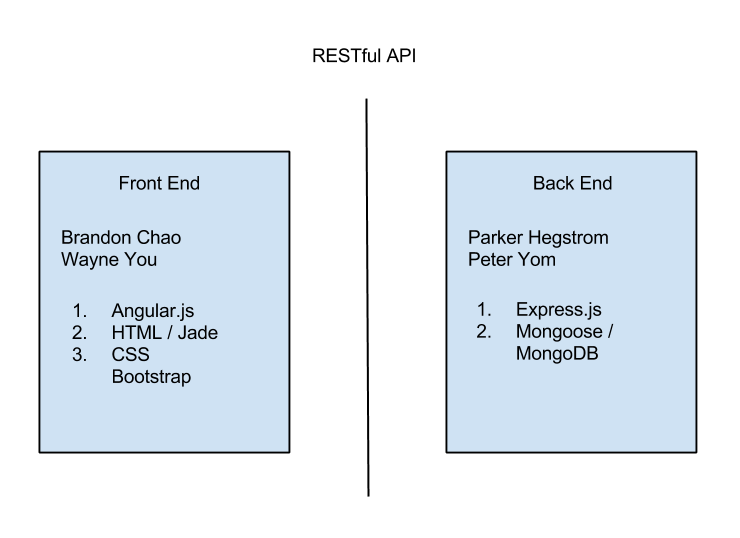
\includegraphics[width=.5\textwidth]{DesignDiagram.png}
\caption{Diagram of our Large Scale Design}
\label{design}
\end{figure}

\noindent Essentially, our back end team provides an exhaustive RESTful API service to our front end. As we received the new requirements for evolution two, the benefits of our modular design came to light as we met to discuss both the refactorings from evolution one that needed to be done and the edits to each modules system design in order to account for the added calendar functionality--event requests and persistent until done events.\\

\noindent At the beginning of evolution three, our group spent four days simply refactoring and making large design change decisions. The back-end did undergo one major change as we now handle repeated events differently. This will be further discussed in the following section.\\

\noindent The following sections further discuss design choices and implications of those design choices for both our front end and back end teams. \\

\section{Back End Design and Analysis}
\subsection{New Features and Developments}
The two new features as well as other design developments are discussed below:
\subsubsection{Slot Sign Up Events}
To implement the slot sign up feature, we created an entirely new structure in the database. This structure, \texttt{SlotSignUp.js}, allowed us to develop without the fear of breaking something already created in the first two evolutions of the project. To handle the dynamic nature of the \texttt{SlotSignUp}, we used the composition design pattern. More specifically, a \texttt{SlotSignUp} is composed of individual \texttt{Slots}, which can be created and associated with any user that signs up for a specific \texttt{Slot}. Initially, though, the \texttt{SlotSignUp} is composed of free blocks of minimum sign up length. As people sign up for slots, the \texttt{Slot} objects are created and tied to that user. This information is stored in the \texttt{attendees} property of the \texttt{SlotSignUp}. \\

\noindent A user must be able to determine the status of the sign up slot (list attendees, what blocks they've signed up for, what free time is left, etc.), and we wanted to make this information as easy as possible to display and edit for the front end. Hence, we stored an attendee's \texttt{email} with his/her slots. This allowed for immediate access to client-ready, displayable information and removed the need for the client to issue additional database queries. Before, the client would have been given a list of user ids and would have had to query the DB with those ids, presenting un-needed latencies to the end user of our application.\\

\noindent Lastly, we wanted the slot sign up to be easily modified or extended in the future, thus was the impetus for using the composition pattern. The \texttt{Slot} was extracted into its own model file and is therefore independent of the \texttt{SlotSignUp}. Say, for example, we wanted to add Alerts to our individual Slots. This would be as easy as creating a new \texttt{Alert} property in \texttt{Slot.js}.

\subsubsection{Find Free Times}

\subsubsection{New Implementation for Repeated Events}
Before, our repeated events were somewhat fake and display driven. We would have one real event in the data base and simply display the event in the future if there was a repeat. We decided we wanted a more powerful approach, one that allowed for repeated events to behave similarly (deleting all at once, sharing same properties) but also behave independently. This new implementation also allowed our code for Find Free Times to run and handle the repeats properly without any additional modification.\\

\noindent To implement this new design, we created a new structure, the \texttt{RepeatChain}. The purpose of this structure was to keep track of all events that were created as a repeat chain, allowing us to edit individual events in the chain as well as delete all repeated events the same time.

\subsubsection{Async.js}
One difficult we've mentioned many times in our discussions and presentations has been the asynchronous nature of javascript. In this evolution, we further implemented a new node module: \texttt{asyn.js}. Under the hood this module works with promises, but this api allowed us control asynchronous dependencies. After witnessing the power of this module, we were able to clean up the call back hell situations we got ourselves into in the past.

\subsubsection{Schema Methods}
Before this evolution, we never used Mongoose Schema methods which leaving our route files cluttered and at times difficult to read. Schema methods allowed us to extract Schema specific behavior and treat our Schemas like classes with an api. For example, we have a \texttt{User} schema. Adding a schema method allowed us to call functions on a \texttt{User} like \texttt{User.convertToEmail()}. Extracting schema methods severely cut back on our repeated code throughout the project. For a working example, see \texttt{./models/User.js}.

\subsection{Benefits of Our Previous Design}
The major benefit of our previous design was its modularity and composition-driven nature. The modularity allowed for easy addition of new features and simultaneous development by all of our team members. It also allowed for easy and testable code as well, because we could test single files or single methods that composed the entire module.\\

\noindent The composition-driven nature of our design proved to be the most powerful thing we've done thus far. That is, we were able to add new features or extend the functionality of previously working code in extremely easy manner, all the while having these changes to database model files persisted throughout the entire database. For example, this evolution required a User to be able to keep track of slots he/she had signed up for or sign up events he/she had created. This was easily done by adding a new property to the Schema Model that ``pointed" to the actual \texttt{Slot} or \texttt{SlotSignUp} objects in the database.

\subsection{Drawbacks of Our Previous Design}
The way we initially design and implemented repeated events proved to be extremely limiting with the new requirements of evolution three. As mentioned before, repeated events used to be simply display-driven, meaning that there was really only one event stored in the data base.\\

\noindent This shortfall was changed such that all repeated events are now actual events in the database.


\section{Front End Design and Analysis}



\section{Individual Portion}
\subsection*{Parker}

\begin{enumerate} [a)]
\item  {\bf Designing and Conducting Experiments}
\begin{enumerate} [$\cdot$]
\item 
\end{enumerate}
\item  {\bf Analyzing and Interpreting Data}
\begin{enumerate} [$\cdot$]
\item  
\end{enumerate}
\item {\bf Designing System Components}
\begin{enumerate} [$\cdot$]
\item 
\end{enumerate}
\item {\bf Dealing with Realistic Contraints}
\begin{enumerate} [$\cdot$]
\item 
\end{enumerate}
\item  {\bf Teamwork and Team Member Interaction}
\begin{enumerate} [$\cdot$]
\item 
\end{enumerate}
\end{enumerate}

\subsection*{Peter}

\begin{enumerate} [a)]
\item  {\bf Designing and Conducting Experiments}
\begin{enumerate} [$\cdot$]
\item 
\end{enumerate}
\item  {\bf Analyzing and Interpreting Data}
\begin{enumerate} [$\cdot$]
\item  
\end{enumerate}
\item {\bf Designing System Components}
\begin{enumerate} [$\cdot$]
\item 
\end{enumerate}
\item {\bf Dealing with Realistic Contraints}
\begin{enumerate} [$\cdot$]
\item 
\end{enumerate}
\item  {\bf Teamwork and Team Member Interaction}
\begin{enumerate} [$\cdot$]
\item 
\end{enumerate}
\end{enumerate}

\subsection*{Brandon}

\begin{enumerate} [a)]
\item  {\bf Designing and Conducting Experiments}
\begin{enumerate} [$\cdot$]
\item An issue I ran into on the frontend while creating the finding free time feature was that even though I was using the same Angular controller for my conflict summary modal and my find free times modal, the scoping of the variables were not the same. In other words, I was not able to access the variables in the scope of the find free times modal from my conflict summary modal. This made it such I could not send the data between the two modals and display the information correctly. I had a hunch that this was due to the second modal not updating the scope when it was rendered which caused it to have an older version of the scope. I tested this by initializing an object and printing it out in both modals after updating it. As I suspected, the object had the new value in the first modal, but an older value in the second modal. I then experimented to see how the scoping could be updated by playing with Angular services. By creating separate controllers and testing out how to share the variables between them, I was able to create a design that had the two modals using separate controllers but with a shared scope through a service. This allowed me to pass the data between the two and display it correctly.
\end{enumerate}
\item  {\bf Analyzing and Interpreting Data}
\begin{enumerate} [$\cdot$]
\item One roadblock we encountered while debugging our finding free times feature was that it was finding the events for users that we didn't specify. We were intrigued by this behavior and discovered that regardless of which users we put in, it was pulling the events for all users. We figured this out by cross referencing the data printed out on the frontend that we were sending into our HTTP request with the data that the backend was receiving in their route. We finally discovered that somewhere in the route, the filter function was working incorrectly which caused the code to pull all users from the calendars instead of using the ones sent in the array from the frontend. We then continued to debug this with print statements in the route which allowed us to check the values of variables with what our expectations of them were. Through this, we ran into some confusing type conversions in Javascript that were turning some of our String variables into Objects and thus making our functions behave differently than expected. We were able to fix these after much trouble and slow debugging as we printed out variables and compared them to the values sent from the frontend and in the database.
\end{enumerate}
\item {\bf Designing System Components}
\begin{enumerate} [$\cdot$]
\item I designed the finding free times feature for this evolution. While the initial modal to find free times is defined in the modalController, functions to display the conflict summary and interact with events are defined in a separate conflictSummaryModalController. We were originally not able to do this since we weren't able to define multiple controllers that needed the same data; however, the Angular services that we discussed above allowed us to share variables between scopes of different controllers which allowed us to split up the controllers into smaller, more specific files. When a free time is found in the conflict summary, I use it to populate the times in the event creation since those variables are stored in the rootScope. From there, I tie this to the modalController and allow the user to create an event and automatically send an invite to each the specified users for this event. 
\end{enumerate}
\item {\bf Dealing with Realistic Contraints}
\begin{enumerate} [$\cdot$]
\item One constraint I encountered in this evolution was the asynchronicity of Javascript. Since the backend team had dealt with this in the past, I originally tried to address this by using the same async library they used. However, I ran into problems with importing the async library and getting it to interact with Angular. I then looked into using promises in Angular and found a function in the \$q Angular library that allows you to make sure one function runs before another function does. This allowed me to complete the finding free times feature since there was an area where I needed to create a new event, and then immediately send invites to users for the event. However, the issue was that the event wasn't being created quickly enough to populate the data used to call the user invite route. This resulted in the route throwing errors from having undefined inputs. After I added the asynchronous control for the order of functions, everything was able to run in the correct order and update as expected.
\end{enumerate}
\item  {\bf Teamwork and Team Member Interaction}
\begin{enumerate} [$\cdot$]
\item For this front-end of this evolution, I worked on the finding free times while Wayne worked on the slot sign ups feature. Since these were very separate features, we did not interact very much throughout the evolution. We met at the beginning of the evolution to plan how we wanted to refactor our code and how we wanted to implement each new feature. Towards the end of the evolution, Peter, Parker, and I met to finish up the evolution. However, Wayne worked remotely and we interacted through messaging. We ran into a lot of problems concerning things that Wayne changed and it was very difficult to debug errors without him working alongside us - especially when he went to sleep before us. We feel like it would be a lot more productive if we worked together near the end of the evolution as we try to tie all of our parts together.
\end{enumerate}
\end{enumerate}

\subsection*{Wayne}

\begin{enumerate} [a)]
\item  {\bf Designing and Conducting Experiments}
\begin{enumerate} [$\cdot$]
\item 
\end{enumerate}
\item  {\bf Analyzing and Interpreting Data}
\begin{enumerate} [$\cdot$]
\item  
\end{enumerate}
\item {\bf Designing System Components}
\begin{enumerate} [$\cdot$]
\item 
\end{enumerate}
\item {\bf Dealing with Realistic Contraints}
\begin{enumerate} [$\cdot$]
\item 
\end{enumerate}
\item  {\bf Teamwork and Team Member Interaction}
\begin{enumerate} [$\cdot$]
\item 
\end{enumerate}
\end{enumerate}

%\keywords{Cremona map \and Newton complementary dual \and monoid \and Cohen--Macaulay}

%\vspace{0.2in}




%\begin{align}
%e^{j\theta} = cos(\theta) + jsin(\theta)
%\end{align}

%\begin{figure}[h]
%\begin{center}
%\epsfig{file=StatPlot.eps, width=5in}
%\caption{\label{boxplot} Box plot of the survey data}
%\end{center}
%\end{figure}


%\begin{figure}[h]
%\begin{center}
%\epsfig{file=histogram.eps, width=4in}
%\caption{\label{histogram} Histogram plot of the survey data}
%\end{center}
%\end{figure}

%\begin{table}[h]
%\begin{center}
%\caption{\label{histotable}Table of frequency values from the Histogram} 
%\begin{tabular}{|c|c|}\hline
%{\bf Type of Engineering} & Frequency \\
%BME & 59 \\
%CEE & 6 \\
%ME & 3 \\
%ECE & 10 \\
%Undecided & 1 \\ \hline
%\end{tabular} \\~\\
%\end{center}
%\end{table}

%\begin{figure}[htb]
%\centering
%\includegraphics[width=1.3\textwidth]{Screenshot.png}
%\caption{Screen shot from StatKey}
%\label{samples}
%\end{figure}


%\appendix
%\section{Codes}
%\subsection{MakeGraph.m}
%\listinginput[1]{1}{MakeGraph.txt}


% GIVES TWO TABLES BY EACHOTHER
%\begin{table}[h!]
%\begin{minipage}[b]{0.45\linewidth}\centering
%\caption{\label{ecoli3}Using {\tt ecoli\_edit\_120481.txt}} 
%\begin{tabular}{|c|c|c|}
%\hline
%1 & 1 & 1 \\
%\hline
%\end{tabular}
%\end{minipage}
%\hspace{0.5cm}
%\begin{minipage}[b]{0.45\linewidth}
%\centering
%\caption{\label{ecoli4}Using {\tt ecoli\_edit\_3947161.txt}} 
%\begin{tabular}{|c|c|c|}
%\hline
%1 & 1 & 1 \\
%\hline
%\end{tabular}
%\end{minipage}
%\end{table}



\end{document}
% end of file template.tex

